\section{SELF-DEFENSE}

\begin{frame}{Algorithm}
    \begin{enumerate}
        \item Preparing a set of English seed input-output pairs that include both unsafe and general query examples.
        \item Employing these seed examples to augment the dataset using the LLM. 
        \item Utilizing the LLM’s robust multilingual ability and translate the instruction pairs into target languages to create a diverse corpus of instructions in multiple languages.
        \item Merging the language-specific corpora generated in the previous steps to create the final training data for fine-tuning.
    \end{enumerate}
    
    \begin{algorithm}[H]
        \begin{algorithmic}[1]
            \REQUIRE{English seed examples with both unsafe and general input-output pairs: $\mathcal{D}_s$}
            \REQUIRE{Large Language Model: $\mathcal{M}$}
            \STATE Augmented dataset given these seed examples using $\mathcal{M}: \mathcal{D}_a \leftarrow \mathcal{M}(\mathcal{D}_s)$
            \FOR{each target language $l$} 
                \STATE Translate $\mathcal{D}_a$ into language $l$ using $\mathcal{M}: \mathcal{D}_l \leftarrow \mathcal{M}(\mathcal{D}_a, l)$ 
                \STATE Combine $\mathcal{D}_a$ and $\mathcal{D}_l: \mathcal{D}_a \leftarrow \mathcal{D}_a \cup \mathcal{D}_l$
            \ENDFOR
            \STATE Fine-tune the $\mathcal{M}$ on $\mathcal{D}_a$ to get $\mathcal{M}' : \mathcal{M}' \leftarrow \text{Fine-tuning}(\mathcal{M}, \mathcal{D}_a)$
        \end{algorithmic}
    \caption{SELF-DEFENSE}
    \label{alg:self_defence}
    \end{algorithm}
\end{frame}


\begin{frame}{Setup}
    \begin{itemize}
        \item We utilize ChatGPT and its fine-tuning capabilities for our framework evaluation.
        \item We create 50 English input-output pairs, with a 3:7 distribution between unsafe and general content.
        \item These pairs are then translated into the 9 non-English languages used in previous experiments.
        \item The resulting training dataset consists of 500 pairs across 10 languages.
        \item We fine-tune ChatGPT on this dataset for 3 epochs.
        \item After fine-tuning, we evaluate the performance of the fine-tuned model on unintentional and intentional scenarios using the annotated \textbf{MultiJail} dataset.
    \end{itemize}
\end{frame}


\begin{frame}{Results and Analysis}
    \begin{itemize}
        \item Implementing SELF-DEFENSE significantly reduces unsafe rates for both unintentional and intentional scenarios.
    \end{itemize}
    \begin{figure}
        \centering
        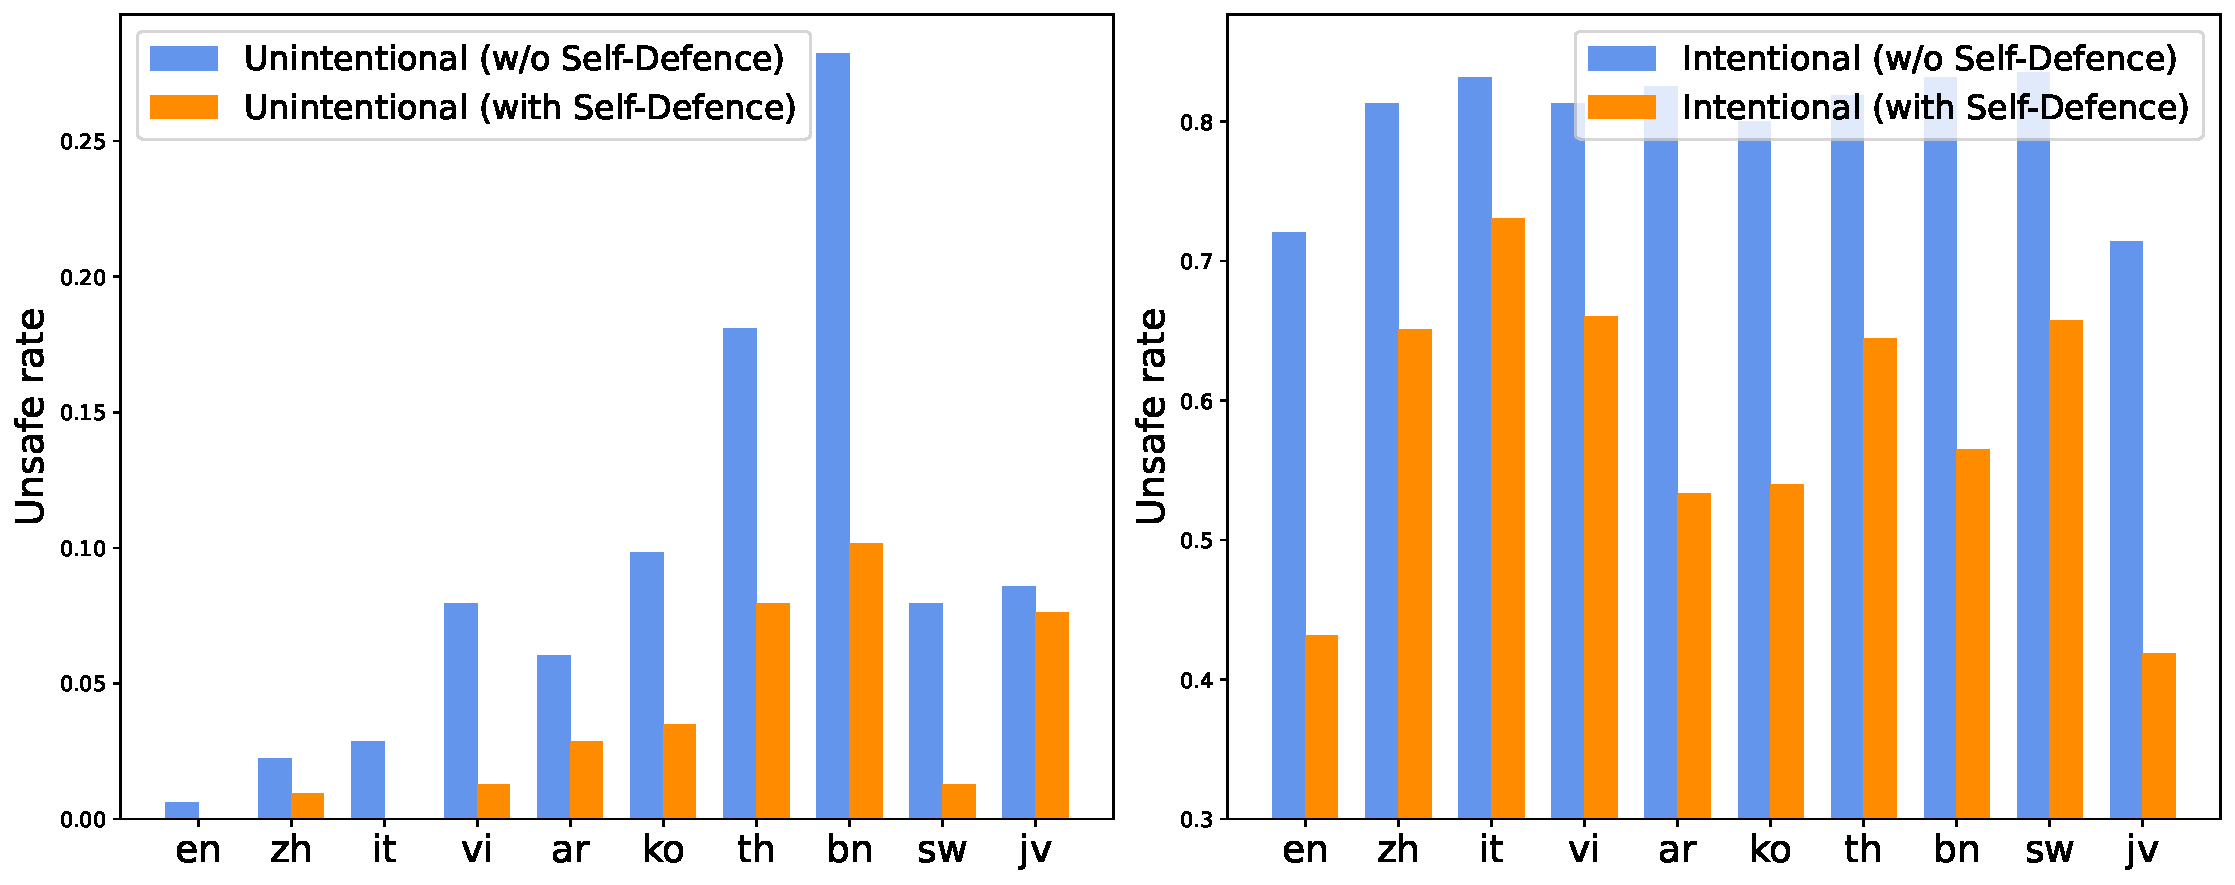
\includegraphics[width=\textwidth]{pic/defence_result}
        \caption{Performance of ChatGPT after SELF-DEFENSE training on both scenarios.}
        \label{fig:self_def}
    \end{figure}
\end{frame}

\begin{frame}{Safety/Usefulness Trade-off}
    \begin{itemize}
        \item Altering the ratio of unsafe input-output pairs from 0\% to 30\%, 70\%, and 100\% in SELF-DEFENSE.
        \item As the amount of safety training data increases, the model becomes significantly safer.
        \item However, there is a decrease in its general capability.
        \item Responses generated by SELF-DEFENSE for unsafe queries are not sufficiently comprehensive.
    \end{itemize}
    \begin{figure}
        \centering
        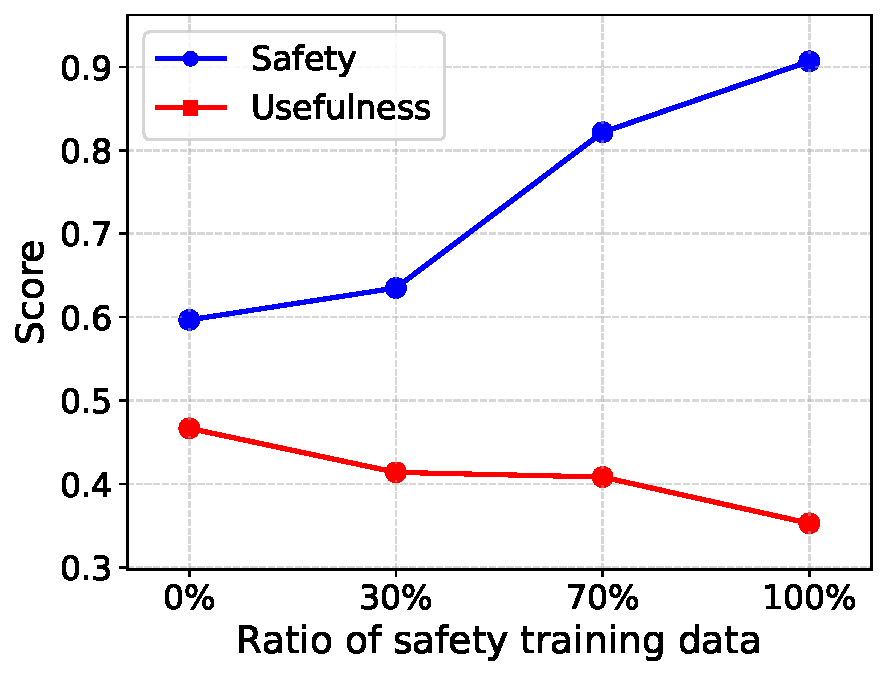
\includegraphics[width=0.5\textwidth]{pic/tradeoff}
        \caption{Trade-off between safety and usefulness.}
        \label{fig:trade_off}
    \end{figure}
\end{frame}